\documentclass[a4paper]{article}
\usepackage[margin=1cm]{geometry}
\usepackage{amsmath, amssymb}
\usepackage{graphicx}
\usepackage{tikz}
\usetikzlibrary{arrows.meta}
\pagestyle{empty}

\definecolor{c0}{HTML}{E53935}
\definecolor{c1}{HTML}{1E88E5}
\definecolor{c2}{HTML}{43A047}
\definecolor{c3}{HTML}{FB8C00}
\definecolor{c4}{HTML}{8E24AA}
\definecolor{c5}{HTML}{00ACC1}
\definecolor{c6}{HTML}{F4511E}
\definecolor{c7}{HTML}{3949AB}
\definecolor{c8}{HTML}{7CB342}
\definecolor{c9}{HTML}{C2185B}
\definecolor{c10}{HTML}{FF7043}
\definecolor{c11}{HTML}{26A69A}
\definecolor{c12}{HTML}{5C6BC0}
\definecolor{c13}{HTML}{FFCA28}
\definecolor{c14}{HTML}{AB47BC}

\begin{document}

\begin{center}
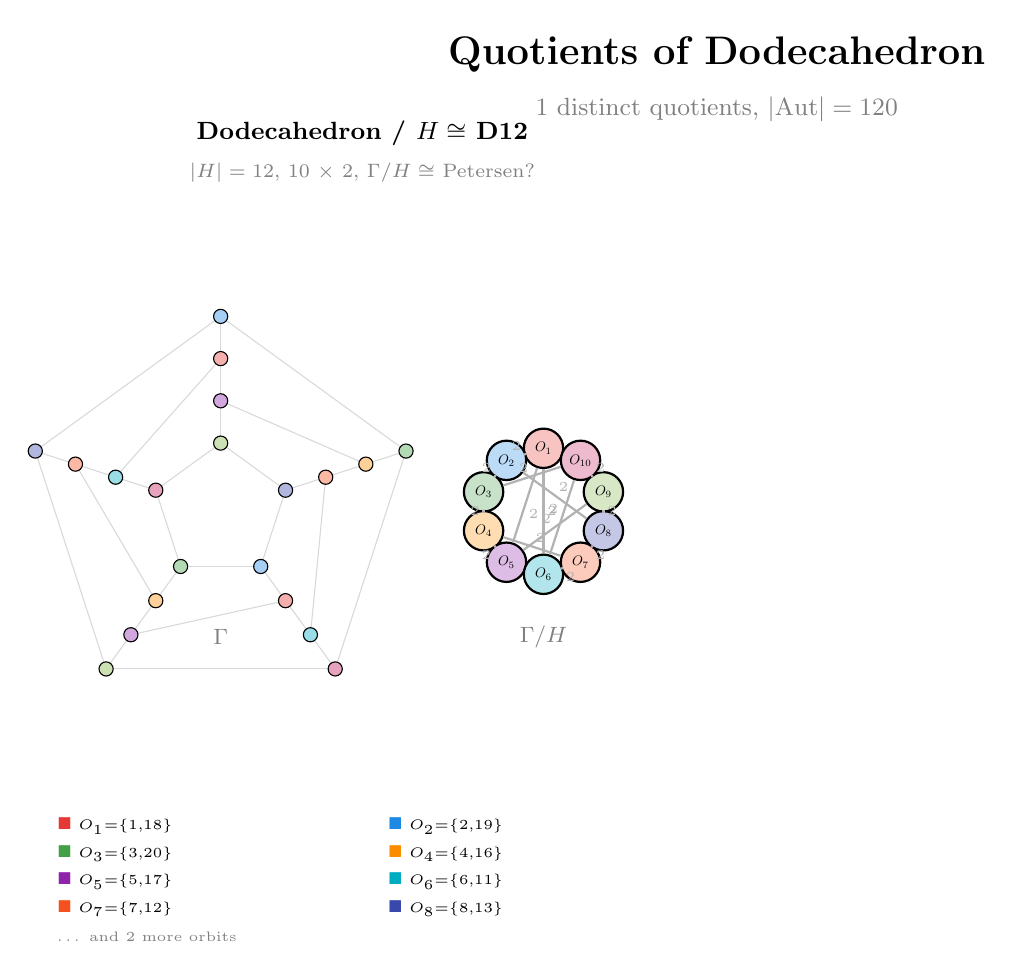
\begin{tikzpicture}[
  ov/.style={circle, draw, semithick, minimum size=3.5mm, inner sep=0pt},
  ovs/.style={circle, draw, thin, minimum size=1.8mm, inner sep=0pt},
  qv/.style={circle, draw, thick, minimum size=5mm, inner sep=0pt},
  cardtitle/.style={font=\small\bfseries},
  cardsub/.style={font=\scriptsize, text=gray},
  glabel/.style={font=\footnotesize, text=gray},
]
\node[font=\Large\bfseries] at (0, 11.5) {Quotients of Dodecahedron};
\node[font=\small, text=gray] at (0, 10.8) {1 distinct quotients, $|\mathrm{Aut}|=120$};

% Card 1: H=D12
\node[cardtitle] at (-4.50,10.50) {Dodecahedron / $H \cong$ D12};
\node[cardsub] at (-4.50,10.00) {$|H|=12$, 10 $\times$ 2, $\Gamma/H \cong$ Petersen?};
\draw[gray!30, thin] (-6.300,7.639) -- (-6.300,8.175);
\draw[gray!30, thin] (-6.300,7.639) -- (-6.300,7.103);
\draw[gray!30, thin] (-6.300,7.639) -- (-7.634,6.133);
\draw[gray!30, thin] (-6.300,8.175) -- (-3.946,6.465);
\draw[gray!30, thin] (-6.300,8.175) -- (-8.654,6.465);
\draw[gray!30, thin] (-3.946,6.465) -- (-4.456,6.299);
\draw[gray!30, thin] (-3.946,6.465) -- (-4.845,3.698);
\draw[gray!30, thin] (-4.456,6.299) -- (-6.300,7.103);
\draw[gray!30, thin] (-4.456,6.299) -- (-4.966,6.133);
\draw[gray!30, thin] (-6.300,7.103) -- (-6.300,6.566);
\draw[gray!30, thin] (-7.634,6.133) -- (-8.144,6.299);
\draw[gray!30, thin] (-7.634,6.133) -- (-7.124,5.968);
\draw[gray!30, thin] (-8.144,6.299) -- (-8.654,6.465);
\draw[gray!30, thin] (-8.144,6.299) -- (-7.124,4.565);
\draw[gray!30, thin] (-8.654,6.465) -- (-7.755,3.698);
\draw[gray!30, thin] (-7.755,3.698) -- (-4.845,3.698);
\draw[gray!30, thin] (-7.755,3.698) -- (-7.440,4.132);
\draw[gray!30, thin] (-4.845,3.698) -- (-5.160,4.132);
\draw[gray!30, thin] (-5.160,4.132) -- (-4.966,6.133);
\draw[gray!30, thin] (-5.160,4.132) -- (-5.476,4.565);
\draw[gray!30, thin] (-4.966,6.133) -- (-5.476,5.968);
\draw[gray!30, thin] (-5.476,5.968) -- (-6.300,6.566);
\draw[gray!30, thin] (-5.476,5.968) -- (-5.791,4.999);
\draw[gray!30, thin] (-6.300,6.566) -- (-7.124,5.968);
\draw[gray!30, thin] (-7.124,5.968) -- (-6.809,4.999);
\draw[gray!30, thin] (-7.124,4.565) -- (-7.440,4.132);
\draw[gray!30, thin] (-7.124,4.565) -- (-6.809,4.999);
\draw[gray!30, thin] (-7.440,4.132) -- (-5.476,4.565);
\draw[gray!30, thin] (-5.476,4.565) -- (-5.791,4.999);
\draw[gray!30, thin] (-5.791,4.999) -- (-6.809,4.999);
\node[ovs, fill=c0!40] at (-6.300,7.639) {};
\node[ovs, fill=c1!40] at (-6.300,8.175) {};
\node[ovs, fill=c2!40] at (-3.946,6.465) {};
\node[ovs, fill=c3!40] at (-4.456,6.299) {};
\node[ovs, fill=c4!40] at (-6.300,7.103) {};
\node[ovs, fill=c5!40] at (-7.634,6.133) {};
\node[ovs, fill=c6!40] at (-8.144,6.299) {};
\node[ovs, fill=c7!40] at (-8.654,6.465) {};
\node[ovs, fill=c8!40] at (-7.755,3.698) {};
\node[ovs, fill=c9!40] at (-4.845,3.698) {};
\node[ovs, fill=c5!40] at (-5.160,4.132) {};
\node[ovs, fill=c6!40] at (-4.966,6.133) {};
\node[ovs, fill=c7!40] at (-5.476,5.968) {};
\node[ovs, fill=c8!40] at (-6.300,6.566) {};
\node[ovs, fill=c9!40] at (-7.124,5.968) {};
\node[ovs, fill=c3!40] at (-7.124,4.565) {};
\node[ovs, fill=c4!40] at (-7.440,4.132) {};
\node[ovs, fill=c0!40] at (-5.476,4.565) {};
\node[ovs, fill=c1!40] at (-5.791,4.999) {};
\node[ovs, fill=c2!40] at (-6.809,4.999) {};
\node[glabel] at (-6.30,4.10) {$\Gamma$};
\node[qv, fill=c0!30] (c0o0) at (-2.200,6.500) {\scalebox{0.5}{$O_{1}$}};
\node[qv, fill=c1!30] (c0o1) at (-2.670,6.347) {\scalebox{0.5}{$O_{2}$}};
\node[qv, fill=c2!30] (c0o2) at (-2.961,5.947) {\scalebox{0.5}{$O_{3}$}};
\node[qv, fill=c3!30] (c0o3) at (-2.961,5.453) {\scalebox{0.5}{$O_{4}$}};
\node[qv, fill=c4!30] (c0o4) at (-2.670,5.053) {\scalebox{0.5}{$O_{5}$}};
\node[qv, fill=c5!30] (c0o5) at (-2.200,4.900) {\scalebox{0.5}{$O_{6}$}};
\node[qv, fill=c6!30] (c0o6) at (-1.730,5.053) {\scalebox{0.5}{$O_{7}$}};
\node[qv, fill=c7!30] (c0o7) at (-1.439,5.453) {\scalebox{0.5}{$O_{8}$}};
\node[qv, fill=c8!30] (c0o8) at (-1.439,5.947) {\scalebox{0.5}{$O_{9}$}};
\node[qv, fill=c9!30] (c0o9) at (-1.730,6.347) {\scalebox{0.5}{$O_{10}$}};
\draw[gray!60, thick] (c0o0) -- node[font=\tiny, auto, inner sep=1pt] {2} (c0o1);
\draw[gray!60, thick] (c0o0) -- node[font=\tiny, auto, inner sep=1pt] {2} (c0o4);
\draw[gray!60, thick] (c0o0) -- node[font=\tiny, auto, inner sep=1pt] {2} (c0o5);
\draw[gray!60, thick] (c0o1) -- node[font=\tiny, auto, inner sep=1pt] {2} (c0o2);
\draw[gray!60, thick] (c0o1) -- node[font=\tiny, auto, inner sep=1pt] {2} (c0o7);
\draw[gray!60, thick] (c0o2) -- node[font=\tiny, auto, inner sep=1pt] {2} (c0o3);
\draw[gray!60, thick] (c0o2) -- node[font=\tiny, auto, inner sep=1pt] {2} (c0o9);
\draw[gray!60, thick] (c0o3) -- node[font=\tiny, auto, inner sep=1pt] {2} (c0o4);
\draw[gray!60, thick] (c0o3) -- node[font=\tiny, auto, inner sep=1pt] {2} (c0o6);
\draw[gray!60, thick] (c0o4) -- node[font=\tiny, auto, inner sep=1pt] {2} (c0o8);
\draw[gray!60, thick] (c0o5) -- node[font=\tiny, auto, inner sep=1pt] {2} (c0o6);
\draw[gray!60, thick] (c0o5) -- node[font=\tiny, auto, inner sep=1pt] {2} (c0o9);
\draw[gray!60, thick] (c0o6) -- node[font=\tiny, auto, inner sep=1pt] {2} (c0o7);
\draw[gray!60, thick] (c0o7) -- node[font=\tiny, auto, inner sep=1pt] {2} (c0o8);
\draw[gray!60, thick] (c0o8) -- node[font=\tiny, auto, inner sep=1pt] {2} (c0o9);
\node[glabel] at (-2.20,4.10) {$\Gamma/H$};
\node[anchor=west, font=\tiny] at (-8.50,1.70) {\textcolor{c0}{$\blacksquare$} $O_{1}$=\{1,18\}};
\node[anchor=west, font=\tiny] at (-4.30,1.70) {\textcolor{c1}{$\blacksquare$} $O_{2}$=\{2,19\}};
\node[anchor=west, font=\tiny] at (-8.50,1.35) {\textcolor{c2}{$\blacksquare$} $O_{3}$=\{3,20\}};
\node[anchor=west, font=\tiny] at (-4.30,1.35) {\textcolor{c3}{$\blacksquare$} $O_{4}$=\{4,16\}};
\node[anchor=west, font=\tiny] at (-8.50,1.00) {\textcolor{c4}{$\blacksquare$} $O_{5}$=\{5,17\}};
\node[anchor=west, font=\tiny] at (-4.30,1.00) {\textcolor{c5}{$\blacksquare$} $O_{6}$=\{6,11\}};
\node[anchor=west, font=\tiny] at (-8.50,0.65) {\textcolor{c6}{$\blacksquare$} $O_{7}$=\{7,12\}};
\node[anchor=west, font=\tiny] at (-4.30,0.65) {\textcolor{c7}{$\blacksquare$} $O_{8}$=\{8,13\}};
\node[anchor=west, font=\tiny, text=gray] at (-8.50,0.30) {\ldots\ and 2 more orbits};
\end{tikzpicture}
\end{center}

\end{document}